\entry{Semana del 26/05/2025}

\section*{Cosas a discutir.}

\begin{itemize}
	\item Por ahí se planchaba por las irregularidades en el alambre de cobre (no recto).
	\item Valor medio de 90°, ¿Por qué?. ¿Mezcladas referencias en Lock-in respecto el output?. 
	\item Tierras distintas del circuito y el agua, ¿aislar la pecera? no sería muy práctico en un canal gigante. 
	\item No variamos la resistencia, a mayor $R$ mayor $Q_F$ y más grande puede ser $\Delta l$. 
	\item La fase $\phi \propto r/e\;\Delta l$, a mayor $e$ o menor $r$ deberíamos aumentar el rango.
	\item Pedir placa de adquisición IO-TECH Personal DAQ 3000 para probar cosas mientras pensamos lo de la Teensy.
	\item Revisar frecuencia de sampleo máxima Raspberry PI
	\item Armar placa PCB con KiCAD:
	
	\begin{itemize}
		\item Potenciómetro en vez de resistencia fija.
		\item 2 x jacks BNC a PCB de 90°, en MercadoLibre pero no la datasheet exacta. Sino comprarlos de antemano para medirlos. Esto para entrada del generador y salida al sensor.
		\item 2 x Borneras de 2 pins para lo mismo (más fácil conseguirlo en ELEMON).
		\item Bornera para voltaje sobre la resistencia o 1 BNC a 2 con las tierras unidas.
		\item Tal vez explorar oscilador 555 a onda sinoiodal con frecuencia variable mediante potenciómetro. 
	\end{itemize}
\end{itemize}


\section{Viernes 30/05/2025} % Miércoles 28/05/2025 

Pedimos prestada la placa, hace falta un transformador AC/DC de 6-16 V y 1A máx para enchufarla, ya que no le alcanza solo con la alimentación de la computadora (no prenden las LEDS), aunque en Ubuntu de la Compu del Labo sí lo reconoce como USB.




\begin{itemize}
	\item Por ahí se planchaba por las irregularidades en el alambre de cobre (no recto).

	Habría que pensar una alternativa, ya sea enderezar el alambre de cobre de alguna forma u otra cosa. Varias ideas serían:
	\begin{itemize}
		\item Extender la impresión hasta abajo del todo, pero no sabemos como afectaría al agua.
		\item Poner varios alambres y promediar, el problema es que todos deberían estar envueltos en agua para que funcione y ya ciertas escalas muy chicas (donde la capilaridad es importante) no se resolverían bien.
	\end{itemize}	
	
	\item Valor medio de 90°, ¿Por qué?. ¿Mezcladas referencias en Lock-in respecto el output?.  
	
	Revisar diagrama de bloques del Lock-in por si agrega la fase, cuál es X y cuál es Y, pero decreció amplitud así que habría que revisarlo.
	
	\item Tierras distintas del circuito y el agua, ¿aislar la pecera? no sería muy práctico en un canal gigante. 
	
	Poner placas grandes para ponerlo a Tierra. Probar agua de la canilla con/sin agregado de sal.
	
	\item No variamos la resistencia, a mayor $R$ mayor $Q_F$ y más grande puede ser $\Delta l$. 
	
	Hay potenciómetros que varían una década.
	
	\item La fase $\phi \propto r/e\;\Delta l$, a mayor $e$ o menor $r$ deberíamos aumentar el rango.
	
	Casi no cambió respecto de la de \cite{gordillozavaletaNonpropagatingHydrodynamicSolitons2012}
	
	\item Pedir placa de adquisición IO-TECH Personal DAQ 3000 para probar cosas mientras pensamos lo de la Teensy.
	
	Ya la fuimos a buscar, falta la potencia, ya que consume más de los 5 V, 0.5 A, que provee la computadora. La compramos, debería llegar el Lunes.
	
	\item Revisar frecuencia de sampleo máxima Raspberry PI.
	
	Llega teóricamente hasta 100 kHz, así que tampoco sería ideal para lo que queremos hacer nosotros.
	
	
	\item Armar placa PCB con KiCAD:
	
	\begin{itemize}
		\item Potenciómetro en vez de resistencia fija.
		\item 2 x jacks BNC a PCB de 90°, en MercadoLibre pero no la datasheet exacta. Sino comprarlos de antemano para medirlos. Esto para entrada del generador y salida al sensor.
		\item 2 x Borneras de 2 pins para lo mismo (más fácil conseguirlo en ELEMON).
		\item Bornera para voltaje sobre la resistencia o 1 BNC a 2 con las tierras unidas.
		\item Tal vez explorar oscilador 555 a onda sinoiodal con frecuencia variable mediante potenciómetro. 
	\end{itemize}
	
	Decidimos armar ambas placas, Ale recomendó para los jacks BNC-PCB de 90° los distribuidores iUrbaNet. % n
	
\end{itemize}

\section{Placas PCB}
Comencé con el diseño de las placas PCB mediante el programa KiCAD.

\begin{figure}[!ht]
	\begin{minipage}[c]{0.5\textwidth}
		\begin{subfigure}{\textwidth}
			\centering
			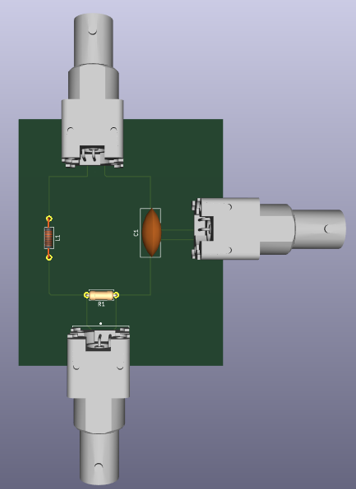
\includegraphics[width=0.65198\textwidth,angle=90,origin=c]{Figures/26_05_2025/PCB_prototipo_BNC}
			\captionsetup{width=0.8\textwidth}
			\subcaption{}
		\end{subfigure}
	\end{minipage}\begin{minipage}[c]{0.49\textwidth}
		\begin{subfigure}{\textwidth}
			\centering
			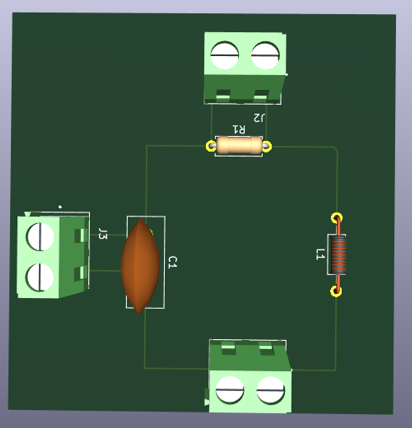
\includegraphics[width=0.78\textwidth]{Figures/26_05_2025/PCB_prototipo_Borneras}
			\captionsetup{width=0.8\textwidth}
			\subcaption{}
		\end{subfigure}
	\end{minipage}
	\caption{Dos vistas del Modelo 3D de la placa con sus componentes.}
	\label{fig:}
\end{figure}





